\documentclass[12pt,a4paper]{report}
\usepackage[utf8]{vietnam} % Sử dụng tiếng việt
\usepackage[top=2cm, bottom=2cm, left=3cm, right=2cm] {geometry} % Canh lề trang
\usepackage{graphicx} % Cho phép chèn hỉnh ảnh
\usepackage{fancybox} % Tạo khung box
\usepackage{indentfirst} % Thụt đầu dòng ở dòng đầu tiên trong đoạn
\usepackage{amsthm} % Cho phép thêm các môi trường định nghĩa
\usepackage{latexsym} % Các kí hiệu toán học
\usepackage{amsmath} % Hỗ trợ một số biểu thức toán học
\usepackage{amssymb} % Bổ sung thêm kí hiệu về toán học
\usepackage{amsbsy} % Hỗ trợ các kí hiệu in đậm
\usepackage{array} % Tạo bảng array
\usepackage{enumitem} % Cho phép thay đổi kí hiệu của list
\usepackage{subfiles} % Chèn các file nhỏ, giúp chia các chapter ra nhiều file hơn
\usepackage{titlesec} % Giúp chỉnh sửa các tiêu đề, đề mục như chương, phần,..
\usepackage{chngcntr} % Dùng để thiết lập lại cách đánh số caption,..
\usepackage{pdflscape} % Đưa các bảng có kích thước đặt theo chiều ngang giấy
\usepackage{afterpage}
\usepackage{capt-of} % Cho phép sử dụng caption lớn đối với landscape page
\usepackage{multirow} % Merge cells
\usepackage{fancyhdr} % Cho phép tùy biến header và footer
\usepackage{setspace}
\usepackage{parskip}
\usepackage[boxruled, lined]{algorithm2e} % Thêm mã giả

\usepackage{times}  % There's an impostor among us =)))

%=======================================================
\usepackage[pdftex, % Sử dụng PDF TeX
bookmarks=true, % Tạo bookmarks trong tập tin PDF
colorlinks=false, % Chữ có màu
pdfencoding=auto, % Tự động điều chỉnh encoding của PDF
unicode=true, % Sử dụng Unicode
pdffitwindow=true, % Fit cho vừa cửa sổ
pdfstartview={FitH}, % Zoom file PDF cho vừa khít với nội dung
pdftoolbar=false, % Ẩn đi tool bar trong PDF viewer
pdfmenubar=false % Ẩn đi menu bar trong PDF viewer
]{hyperref}


% Phụ lục 
\usepackage[toc,page]{appendix} % Thêm phụ lục
\renewcommand{\appendixname}{Phụ lục}
\renewcommand{\appendixtocname}{Phụ lục}
\renewcommand{\appendixpagename}{Phụ lục}

% Tài liệu tham khảo
\usepackage[backend=biber]{biblatex}
\addbibresource{bibliography/report-bib.bib}
\DefineBibliographyStrings{english}{%
bibliography = {Tài liệu tham khảo},
references = {Tài liệu tham khảo},
}



% Dãn cách dòng & đánh số phần
\onehalfspacing
\setlength{\parskip}{6pt}
\setlength{\parindent}{15pt}
\renewcommand{\baselinestretch}{1.5}
\renewcommand{\thesection}{\arabic{section}}


% Tên và tác giả
\def \TITLE{Các phương pháp tìm gần đúng ma trận nghịch đảo}
\def \AUTHOR{\textbf{Bùi Tiến Thành - MSSV 20190081}  \\\textbf{Chu Thị Ngân - MSSV 20195904} \\}
\date{Tháng Mười một, 2020}


% Đầu trang và chân trang
\pagestyle{fancy}
\fancyhf{}
\lhead{\rightmark}
\rfoot{CTTN Toán tin K64 }
\lfoot{Bùi Tiến Thành \texttt{(thanh.bt190081@sis.hust.edu.vn)} \\Chu Thị Ngân \texttt{(ngan.ct195904@sis.hust.edu.vn)}}
\rhead{Trang \thepage}
\renewcommand{\headrulewidth}{2pt}
\renewcommand{\footrulewidth}{2pt}


% Hình vẽ
\graphicspath{{./rpt-img/}}




%=======================================================
\begin{document}

    \newgeometry{top=2cm, bottom=2cm, left=3cm, right=2cm}
    \begin{titlepage}
    \thispagestyle{empty}
    \thisfancypage{
    \setlength{\fboxsep}{3pt}
    \fbox}{} 

    \begin{center}
    \vspace{3cm}
    {\bf\large ĐẠI HỌC BÁCH KHOA HÀ NỘI}\\
    {\bf VIỆN TOÁN ỨNG DỤNG VÀ TIN HỌC}\\[2cm]
    
    \begin{center}
        
\includegraphics[scale=0.2]{LOGO_HUST.png}
    \end{center}
    
    
    \vspace{2cm}
    {\bf\Large CÁC PHƯƠNG PHÁP}\\
    {\bf\Large TÌM GẦN ĐÚNG MA TRẬN NGHỊCH ĐẢO}\\
    
    \vspace{1cm}
    {\bf \AUTHOR}
    
    \vspace{1cm}
    {\bf GIẢNG VIÊN HƯỚNG DẪN}\\
    {\bf TS. Hà Thị Ngọc Yến}
    \end{center}
    
    \vspace{6cm}
    \begin{center}
    {\bf Hà Nội, tháng 11, 2020}
    \end{center}

\end{titlepage}
    \restoregeometry

    \pagestyle{empty}
    \newpage
    \addcontentsline{toc}{section}{\protect\numberline{}Mục lục}
    \tableofcontents
    \newpage

    \pagestyle{fancy}

    \section{Đặt vấn đề}
    \subsection{Phái biểu bài toán}
        \par \textbf{Bài toán: } Cho ma trận $A$ vuông cấp n, khả nghịch. Tìm ma trận nghịch đảo của $A$.

        \par Trong báo cáo này, nhóm sẽ nghiên cứu các phương pháp giải gần đúng nghịch đảo của ma trận trên ma trận thực vuông cấp $n$, khả nghịch. Nói cách khác, ta có ma trận $ A $ thỏa mãn các tính chất sau:

        $$ A \in \mathbf{M}_{n*n} (\mathbb{R}) \text{  và  } det(A) \neq 0 $$ 

        \par ở đó $ \mathbf{M}_{n*n} (\mathbb{R}) $ là tập các ma trận vuông cấp n trên tập số thực.
            
    \subsection{Tại sao phải giải gần đúng?}
        \par Các phương pháp giải chính xác thường cho ra lời giải sau hữu hạn bước và thậm chí cho lời giải chính xác nếu máy tính có thể xử lý số thực với cấp chính xác là vô cùng. Tuy nhiên, các phương pháp này gặp khó khăn với những ma trận có kích thước rất lớn và có nhiều phần tử không (hay còn gọi là ma trận thưa) và do hạn chế của tính toán số trên máy tính, các phương pháp giải đúng có thể sinh ra sai số rất lớn. Hơn nữa, độ phức tạp cúa các phương pháp tìm chính xác ma trận nghịch đảo là $\mathcal{O} (n^{3})$ và khối lượng tính toán sẽ tăng rất nhanh khi tăng kích cỡ ma trận. Do đó, phương pháp xấp xỉ được phát minh để phần nào giải quyết những vấn đề mà phương pháp chính xác gặp phải. 
            
    \subsection{Các phương pháp giải}
        \par Ta thấy đây là một trường hợp riêng của bài toán giải phương trình $ A X = B $, trong đó $B = E $ là ma trận đơn vị cấp $n$, do đó có thể áp dụng các phương pháp giải gần đúng phương trình ma trận vào bài toán này. Ngoài ra, nhóm còn đề cập thêm một phương pháp riêng là phương pháp Newton để tìm gần đúng ma trận nghịch đảo.

        \begin{enumerate}[label = (\roman*)]
            \item Phương pháp Newton
            \item Phương pháp lặp đơn và lặp Jacobi
            \item Phương pháp lặp Gauss-Seidel
        \end{enumerate}

    \subsection{Chuẩn ma trận và sự hội tụ của dãy ma trận}
        \par Điểm chung của các phương pháp này là đều xuất phát từ một xấp xỉ ban đầu $X^{(0)}$, tìm cách hiệu chỉnh dần sau một số bước ta thu được dãy  $ \{ X^{(k)} \} $ mà $ \{ X^{(k)} \} $ tiến gần đến $A^{-1}$. Do đó, cần đưa vào khái niệm về chuẩn và sự hội tụ của dãy ma trận
            
        \par \textbf{Về chuẩn của ma trận:} Trong báo cáo này, nhóm sẽ sử dụng một số chuẩn thông dụng để xác định sai số và độ hội tụ của các phương pháp. Các chuẩn đó là chuẩn Euclid (chuẩn 2), chuẩn cột (chuẩn 1) và chuẩn hàng (chuẩn vô cùng) và chúng được định nghĩa như sau:
        
        $$ \left\lVert A \right\rVert_{2} = \sqrt{ \sum\limits_{1}^{n} \sum\limits_{1}^{n} \left\lvert A_{ij} \right\rvert^{2}  }   $$
        $$ \left\lVert A \right\rVert_{1} = \max\limits_{1 \leq j \leq n} \sum\limits_{i = 1}^{n} \left\lvert A_{ij} \right\rvert    $$
        $$ \left\lVert A \right\rVert_{\infty} =  \max\limits_{1 \leq i \leq n} \sum\limits_{j = 1}^{n} \left\lvert A_{ij} \right\rvert $$

        Dễ thấy các "chuẩn" này là một chuẩn trên $ \mathbf{M}_{n*n} (\mathbb{R}) $ và thỏa mãn các tiên đề của chuẩn \textit{(bạn đọc tự chứng minh như một câu hỏi)}

        \par \textbf{Sự hội tụ của dãy ma trận:} Từ chuẩn của ma trận, ta xây dựng định nghĩa về sự hội tụ của dãy ma trận như sau: Dãy ma trận $ \{ A^{(k)} \} \subset \mathbf{M}_{n*n} (\mathbb{R}) $ hội tụ về ma trận $ A $, hay $ \lim_{k \to \infty} A^{(k)} = A $ nếu:

        $$ \lim_{k \to \infty} \left\lVert A^{(k)} - A \right\rVert = 0 $$


    
    \section{Phương pháp Newton}
        
    \subsection{Ý tưởng}
        \par Giả sử cho số thực $a$ khác 0 , tìm $x$ để $ax = 1 \Rightarrow a = \frac{1}{x}$ với $a \neq 0$. Ta đặt:

        $$ f(x) = a - \frac{1}{x} = 0 $$

        \par Theo công thức Newton:

        $$ x_{k+1} = x_{k} - \frac{f(x_{k})}{f'(x_{k})} = x_{k} - \frac{a - \frac{1}{x_{k}}}{\frac{1}{x_{k}^{2}}} $$

        \par hay: 
            
        $$ x_{k+1} = x_{k}(2 - ax_{k}) \text{ với } k \in \mathbb{N} $$
        
    \subsection{Công thức lặp}
        \par Vận dụng ý tưởng trên, xem $a$ là ma trận $A$, $x$ là ma trận $X$, cần tìm $X$ sao cho $ A X = X A = E $ ta có công thức lặp như sau:
            
        \begin{equation}
            X_{k+1} = X_{k}(2E - AX_{k}) \text{  với  } k \in \mathbb{N} 
        \end{equation}

        \par ở đó $E$ là ma trận đơn vị cùng cấp và $X_{0}$ là xấp xỉ đầu

    \subsection{Điều kiện hội tụ}
        \par Ta cần tìm điều kiện để 
        $$ \lim_{k \to \infty} X_{k} = A^{-1} $$
        
        \par Ta đặt $ G_{k} = E - AX_{k} $. Theo công thức $(1)$ ta được:
        \begin{align*}
            G_{k} &= E - AX_{k-1}(2E - AX_{k-1}) \\
                  &= E - 2AX_{k-1} + (AX_{k-1})^{2} \\
                  &= (E - AX_{k-1})^{2} = G_{k-1}^{2} 
        \end{align*}
        
        \par Theo truy hồi ta có: $ G_{k} = G_{k-1}^{2} = (G_{k-2}^2)^2 = (G_{k-2})^4 = ...... = G_{0}^{2^{k}} $
        
        \par Mặt khác $A^{-1} - X_{k} = A^{-1}(E - AX_{k}) = A^{-1}G_{k} = A^{-1}G_0^{2^{k}}$ nên:
        \begin{equation}
            \left\lVert A^{-1} - X_{k} \right\rVert \leq \left\lVert A^{-1} \right\rVert \left\lVert G_{0} \right\rVert ^{2^{k}}
        \end{equation}
        \par ở đó $ G_{0} = E - AX_{0} $. Cũng từ $(2)$ ta thấy nếu $\left\lVert G_{0} \right\rVert < 1 $ thì:

        $$ \left\lVert A^{-1} - X_{k} \right\rVert \xrightarrow{k \to \infty} 0 \text{  hay  } \lim_{k \to \infty} X_{k} = A^{-1}  $$

        Vậy $\left\lVert G_{0} \right\rVert < 1$ là điều kiện để quá trình lặp $(1)$ hội tụ. Tuy nhiên, trên máy tính ta không thể cho k lặp đến vô cùng mà chỉ lặp đến một khoảng sai số nhất định nên vì vậy, cần phải xây dựng công thức sai số.

    \subsection{Công thức sai số}
        Giả sử $ \left\lVert G_{0} \right\rVert \leq q < 1 $. Ta lại có:
        \begin{align*}
            G_{0} = E - AX_{0} &\Leftrightarrow X_{0} = A^{-1}(E - G_{0}) \\
                               &\Leftrightarrow A^{-1} = X_{0}(E - G_{0})^{-1} \\
                               &\Leftrightarrow A^{-1} = X_{0}(E + G_{0} + G_{0}^{2} + .....) \\
        \end{align*} 
        \par Suy ra $ \Rightarrow \left\lVert A^{-1} \right\rVert \leq \left\lVert X_{0} \right\rVert (1 + q + q^{2} + ....) = \frac{\left\lVert X_{0} \right\rVert}{1 - q} $

        \par Thay vào $(2)$ ta được:
        $$ \left\lVert A^{-1} - X_{k} \right\rVert \leq \frac{\left\lVert X_{0} \right\rVert}{1 - q} \left\lVert G_{0} \right\rVert ^{2^{k}} = \frac{\left\lVert X_{0} \right\rVert}{1 - q} q^{2^{k}} $$

        Từ đó ta có công thức đánh giá sai số như sau:
        \begin{equation}
            \left\lVert A^{-1} - X_{k} \right\rVert \leq \frac{\left\lVert X_{0} \right\rVert}{1 - q} q^{2^{k}} 
        \end{equation}
            
    \subsection{Thuật toán và chương trình}
        \subsubsection{Input, Output và chương trình:} 
            \par \textbf{Input:} Ma trận $A$, xấp xỉ đầu $X_{0}$ và sai số $\varepsilon$. Giả thiết coi như các công thức ở \textbf{2.3} và \textbf{2.4} thỏa mãn
            \par \textbf{Output:} Ma trận xấp xỉ $A^{-1}$
            % \par \textbf{Chương trình: }\href{https://github.com/bu1th4nh/TALENTED-K64MI/tree/master/MI3040/report-code/Newton}{\texttt{lib\_newton.py}}


        \subsubsection{Mã giả:}
            \IncMargin{1em}\begin{algorithm}[H]
                \caption{Phương pháp Newton tìm ma trận nghịch đảo \label{IR}}
                \KwIn{Ma trận $A, X_{0}, \varepsilon$}
                \KwOut{Ma trận $X^{*} = A^{-1}$ là ma trận nghịch đảo}
                \SetAlgoLined     
                \Begin{
                    Nhập $A, X_{0}, \varepsilon$\;
                    
                    $ q \longleftarrow \left\lVert E - AX_{0} \right\rVert $\;
                    $ k \longleftarrow 0 $\;
                    $ X \longleftarrow X_{0}   $\;
                    
                    \While{$ \frac{\left\lVert X_{0} \right\rVert * q^{2^{k}} }{1 - q} > \varepsilon $}{    
                        $ X \longleftarrow X(2E - AX) $\;
                        $ k \longleftarrow k + 1 $\;
                        }
                        
                    Đưa ra $X$ chính là ma trận nghịch đảo\;
                }       
            \end{algorithm}\DecMargin{1em}


        \subsubsection{Giải thích biến trong thuật toán:}
            \begin{itemize}
                \item $A$: Ma trận cần nghịch đảo
                \item $X_{0}$: Xấp xỉ đầu vào
                \item $\varepsilon$: Sai số cho phép
                \item $E$: Ma trận đơn vị cùng cấp với $A$
                \item $X$: Dãy ma trận $X_{k}$, tuy nhiên chúng ta chỉ cần xét phần tử $X_{n-1}$ để tính $X_{k}$ nên chúng ta chỉ cần 1 ma trận $X$
                \item $q$: Giá trị q trong công thức sai số
            \end{itemize}

            




    \section{Phương pháp lặp Jacobi}
\subsection{Công thức lặp}
    Như kiến thức đã biết trong phần lặp Jacobi, với $ T = diag\{\frac{1}{A_{11}}, \frac{1}{A_{22}},..., \frac{1}{A_{nn}}\} $ là ma trận đường chéo cấp n, ta có:

    \begin{equation}
        X_{k+1} = (E - TA)X_{k} + T 
    \end{equation}

    Do phần này \textit{(cùng với phương pháp lặp Gauss-Seidel)} nằm trong phần kiến thức đã biết nên trong báo cáo chỉ áp dụng trực tiếp và không chứng minh các công thức.

\subsection{Điều kiện hội tụ}

    \hypertarget{jacobi.math.convergence}{Phương pháp này} cùng với phương pháp lặp Gauss-Seidel \textit{(sẽ được nêu sau)} hội tụ nếu $ \left\lVert E - TA \right\rVert < 1 $, tức là ma trận A phải chéo trội:
    
    $$\sum\limits_{j = 1, j \neq i}^{n} \left\lvert A_{ij} \right\rvert < \left\lvert A_{ii}\right\rvert \; \forall i = \overline{1,n} \; \; \text{\textit{(chéo trội hàng)}} $$

    $$\text{ hoặc }  \sum\limits_{i = 1, i \neq j}^{n} \left\lvert A_{ij} \right\rvert < \left\lvert A_{jj}\right\rvert \; \forall j = \overline{1,n}  \; \; \text{\textit{(chéo trội cột)}}$$

\subsection{Công thức sai số}

    Ta vẫn đặt $ T = diag\{\frac{1}{A_{11}}, \frac{1}{A_{22}},..., \frac{1}{A_{nn}}\} $ như trong phần 3.2. Ta xét 2 trường hợp:

    \begin{enumerate}[label = (\roman*)]
        \item \textbf{Trường hợp chéo trội hàng:} Đặt $B = E - TA$, dễ thấy tồn tại một số $q$ để:
        
        $$ \left\lVert B\right\rVert _{\infty} \leq q < 1 $$ 
        
        Do đó, ta có công thức sai số như sau:
        
        \begin{equation}
            \left\lVert X_{k} - X^{*} \right\rVert_{\infty} \leq \frac{q}{1 - q} \left\lVert X_{k} - X_{k - 1} \right\rVert_{\infty} \\
        \end{equation}
        \begin{equation}
            \left\lVert X_{k} - X^{*} \right\rVert_{\infty} \leq \frac{q^{k}}{1 - q} \left\lVert X_{1} - X_{0} \right\rVert_{\infty}
        \end{equation}


        \item \textbf{Trường hợp chéo trội cột:} Đặt $B_{1} = E - AT$ và $\lambda = \frac{max \left\lvert A_{ii}\right\rvert }{min \left\lvert A_{ii}\right\rvert }, \left\lVert B_{1}\right\rVert _{1} \leq q < 1 $, dễ thấy tồn tại một số $q$ để:
        
        $$ \left\lVert B_{1} \right\rVert _{1} \leq q < 1 $$ 
        
        Do đó, ta có công thức sai số như sau:
        
        \begin{equation}
            \left\lVert X_{k} - X^{*} \right\rVert_{1} \leq \lambda \frac{q}{1 - q} \left\lVert X_{k} - X_{k - 1} \right\rVert_{1}
        \end{equation}
        \begin{equation}
            \left\lVert X_{k} - X^{*} \right\rVert_{1} \leq \lambda \frac{q^{k}}{1 - q} \left\lVert X_{1} - X_{0} \right\rVert_{1}
        \end{equation}

    \end{enumerate}

\subsection{Thuật toán và chương trình}
%=====================================================================================%
%                                     MAIN ALGO                                       %
%=====================================================================================%
    \hypertarget{jacobi.algo}{\textbf{Mã giả thuật toán chính: }}   \\
    \IncMargin{1em}\begin{algorithm}[H]
        \caption{Phương pháp Jacobi tìm ma trận nghịch đảo \label{IR}}
        \KwIn{Ma trận $A$ chéo trội, sai số $\varepsilon$}
        \KwOut{Ma trận $X^{*} = A^{-1}$ là ma trận nghịch đảo}
        \SetAlgoLined   
        \Begin{
            Nhập $A, \varepsilon$\;
            \BlankLine
            $ p \longleftarrow $ \hyperlink{jacobi.checkDom}{checkDomination}$(A) $\;
            $ T \longleftarrow diag\{ \frac{1}{A_{11}}, \frac{1}{A_{22}}, ..., \frac{1}{A_{nn}} \} $\;
            $ B \longleftarrow E - TA, B_{1} \longleftarrow E - AT$\;
            $ q \longleftarrow $ \hyperlink{jacobi.getNorm}{getNorm}$(B,B_{1}, p) $\;
            $ \lambda \longleftarrow $ \hyperlink{jacobi.getLambda}{getLambda}$(A, p) $\;
            \BlankLine
            $ X^{*} \longleftarrow $ \hyperlink{jacobi.iterate}{iterate}$(X_0 \leftarrow A, B, T, q, \lambda, p, \varepsilon) $\;
            Trả về $X^{*}$ là ma trận nghịch đảo\;
        }         
    \end{algorithm}\DecMargin{1em}

%=====================================================================================%
%                                        NORM                                         %
%=====================================================================================%
    \hypertarget{jacobi.getNorm}{\textbf{Gói chọn chuẩn}}   \\
    \IncMargin{1em}\begin{function}[H]
        \caption{getNorm(A, $A_{1}$, p)}
        \KwIn{Ma trận $A$, giá trị kiểm tra $p$}
        \KwOut{ $ \left\lVert A \right\rVert_{\infty}  $ nếu $p = 1$, $ \left\lVert A_{1} \right\rVert_{1}  $ nếu $p = -1$}
        \Begin{
            \lIf{$ p = 1 $}{\KwRet{$\left\lVert A \right\rVert_{\infty}$}}
            \lIf{$ p = -1 $}{\KwRet{$\left\lVert A_{1} \right\rVert_{1}$}}
        }
    \end{function}\DecMargin{1em}
    
\newpage
%=====================================================================================%
%                                     CHECK DOM                                       %
%=====================================================================================%
    \hypertarget{jacobi.checkDom}{\textbf{Gói kiểm tra ma trận chéo trội}} \\
    \IncMargin{1em}\begin{function}[H]
        \caption{checkDomination(A)}
        \KwIn{Ma trận $A$}
        \KwOut{Giá trị kiểm tra $p$ bằng 1 nếu $A$ chéo trội hàng, -1 nếu $A$ chéo trội cột, 0 khi $A$ không chéo trội}
        \Begin{
            $ row\_dom \longleftarrow 1 $, $ col\_dom \longleftarrow 1 $ \;
            \For{$i=1$ \KwTo n}{
                \lIf{ $ \sum\limits_{j = 1, j \neq i}^{n} \left\lvert A_{ij} \right\rvert >= \left\lvert A_{ii}\right\rvert $ }{ $ row\_dom \longleftarrow 0 $}
                \lIf{ $ \sum\limits_{j = 1, j \neq i}^{n} \left\lvert A_{ji} \right\rvert >= \left\lvert A_{ii}\right\rvert $ }{ $ col\_dom \longleftarrow 0 $}
            }
            \BlankLine
            \lIf{$ row\_dom = 1 $}{\KwRet{1}}
            \lIf{$ col\_dom = 1 $}{\KwRet{-1}}
            \KwRet{0} \;
        }
    \end{function}\DecMargin{1em}

%=====================================================================================%
%                                       LAMBDA                                        %
%=====================================================================================%
    \vspace{2cm}
    \hypertarget{jacobi.getLambda}{\textbf{Gói chọn giá trị lambda}} \\
    \IncMargin{1em}\begin{function}[H]
        \caption{getLambda(A, p)}
        \KwIn{Ma trận $A$, giá trị kiểm tra $p$}
        \KwOut{ $ \lambda = 1 $ nếu $p = 1$, $ \lambda = \frac{max \left\lvert A_{ii}\right\rvert }{min \left\lvert A_{ii}\right\rvert } $ nếu $p = -1$}
        \Begin{
            \lIf{$ p = 1 $}{\KwRet{1}}
            \BlankLine
            $ max\_A \longleftarrow \left\lvert A_{11} \right\rvert  $\;
            $ min\_A \longleftarrow \left\lvert A_{11} \right\rvert  $\;
            \For{$i=1$ \KwTo n}{
                $ max\_A = max(max\_A, \left\lvert A_{ii} \right\rvert ) $\;
                $ min\_A = min(min\_A, \left\lvert A_{ii} \right\rvert ) $\;
            }
            \KwRet{$\frac{max\_A}{min\_A}$}
        }
    \end{function}\DecMargin{1em}


\newpage
%=====================================================================================%
%                                     ITERATION                                       %
%=====================================================================================%
    \hypertarget{jacobi.iterate}{\textbf{Gói lặp - Đánh giá tiên nghiệm}} \\
    \IncMargin{1em}\begin{function}[H]
        \caption{iterate($X_{0}, B, T, q, \lambda, p, \varepsilon$)}
        \KwIn{Ma trận xấp xỉ đầu $X_{0}$, $B$, $T$, hệ số $q$, $\lambda$, giá trị kiểm tra $p$ và sai số $\varepsilon$}
        \KwOut{$X^{*}$ là ma trận nghịch đảo theo đánh giá tiên nghiệm}
        \Begin{
            $qk \longleftarrow 1, X \longleftarrow X_{0}$ \;
            $predecessor\_norm \longleftarrow$ \hyperlink{jacobi.getNorm}{getNorm}$((BX_{0} + T) - X_{0}, p)$ \;
            \BlankLine
            \While{$ \frac{\lambda * qk * predecessor\_norm}{1 - q} > \varepsilon $}{
                $ X \longleftarrow BX + T $ \;
                $ qk \longleftarrow qk * q $ \;
            }
            \BlankLine
            \KwRet{X}
        }
    \end{function}\DecMargin{1em}
    
    \vspace{1cm}
    \par \textbf{Gói lặp - Đánh giá hậu nghiệm }\\
    \IncMargin{1em}\begin{function}[H]
        \caption{iterate($X_{0}, B, T, q, \lambda, p, \varepsilon$)}
        \KwIn{Ma trận xấp xỉ đầu $X_{0}$, $B$, $T$, hệ số $q$, $\lambda$, giá trị kiểm tra $p$ và sai số $\varepsilon$}
        \KwOut{$X^{*}$ là ma trận nghịch đảo theo đánh giá hậu nghiệm}
        \Begin{
            $old\_X \longleftarrow X_{0} $\;
            $new\_X \longleftarrow BX_{0} + T $\;

            \BlankLine
            \While{$ \frac{\lambda * q * \text{\hyperlink{jacobi.getNorm}{getNorm}}(new\_X - old\_X, p)}{1 - q} > \varepsilon $}{
                $ old\_X \longleftarrow new\_X $\;
                $ new\_X \longleftarrow B * old\_X + T $\;
            }
            \BlankLine

            \KwRet{$new\_X$}
        }
    \end{function}\DecMargin{1em}

    
\par \textbf{Chương trình: }\href{https://github.com/Talented-K64MI/MI3040-Numerical-Analysis/tree/master/Topic%202.5%20-%20Matrix%20Inversion/Jacobi%20Method}{\texttt{jacobi.py}}
\newpage



    \section{Phương pháp Gauss - Seidel}
    \par Phương pháp Gauss-Seidel là một cải tiến theo ý tưởng của phương pháp lặp đơn và Jacobi, cho phép tính toán theo dòng của ma trận từ đó tiết kiệm bộ nhớ hơn các phương pháp thông thường. Do phần này \textit{(cùng với phương pháp lặp Jacobi)} nằm trong phần kiến thức đã biết nên trong báo cáo chỉ áp dụng trực tiếp và không chứng minh các công thức. Phần này cũng không nêu điều kiện hội tụ bởi điều kiện hội tụ của phương pháp này hoàn toàn tương tự như \hyperlink{jacobi.math.convergence}{phương pháp Jacobi.}


\subsection{Công thức lặp}
    \par Đặt $B = E - TA$ với $T = diag\{\frac{1}{A_{11}}, \frac{1}{A_{22}},..., \frac{1}{A_{nn}}\} $ tương tự như trên. Như kiến thức đã biết trong phần lặp Gauss-Seidel, ta có công thức lặp sau\cite{giaotrinhgiaitichso}:

    \begin{equation}
        X_{i}^{(k+1)} = \sum\limits_{j=1}^{i-1} B_{ij}X_{j}^{(k+1)} + \sum\limits_{j=i+1}^{n} B_{ij}X_{j}^{(k)} + T_{i}
    \end{equation}
    với mọi $i = \overline{1,n}$ và $A_{i}$ là dòng $i$ của ma trận $A$

\subsection{Công thức sai số}

    Ta vẫn đặt $ T = diag\{\frac{1}{A_{11}}, \frac{1}{A_{22}},..., \frac{1}{A_{nn}}\} $ như trong phần 3.2. Ta xét 2 trường hợp:

    \begin{enumerate}[label = (\roman*)]
        \item \textbf{Trường hợp chéo trội hàng:} Đặt $B = E - TA$, dễ thấy tồn tại một số $q$ để:
        
        $$ q = \max\limits_{1 \leq i \leq n} \frac{\sum\limits_{j=i}^{n} \left\lvert B_{ij} \right\rvert}{1 - \sum\limits_{j=1}^{i-1} \left\lvert B_{ij} \right\rvert} \leq \left\lVert B \right\rVert_{\infty} < 1 $$
        
        Do đó, ta có công thức sai số như sau:
        
        \begin{equation}
            \left\lVert X_{k} - X^{*} \right\rVert_{\infty} \leq \frac{q}{1 - q} \left\lVert X_{k} - X_{k - 1} \right\rVert_{\infty}
        \end{equation}
        \begin{equation}
            \left\lVert X_{k} - X^{*} \right\rVert_{\infty} \leq \frac{q^{k}}{1 - q} \left\lVert X_{1} - X_{0} \right\rVert_{\infty}
        \end{equation}

        \newpage

        \item \textbf{Trường hợp chéo trội cột:} Đặt $B_{1} = E - AT$, ta có:
        
        $$ q = \max\limits_{1 \leq i \leq n} \frac{\sum\limits_{j=1}^{i} \left\lvert B_{1_{ji}} \right\rvert}{1 - \sum\limits_{j=i+1}^{n} \left\lvert B_{1_{ji}} \right\rvert} \leq \left\lVert B_{1} \right\rVert_{1} < 1 $$ 
        $$ S = \max\limits_{1 \leq i \leq n} \sum\limits_{j=i+1}^{n} \left\lvert B_{1_{ji}} \right\rvert $$
        
        Do đó, ta có công thức sai số như sau\cite{giaotrinhgiaitichso}: 
        
        \begin{equation}
            \left\lVert X_{k} - X^{*} \right\rVert_{1} \leq \frac{q}{(1 - S)(1 - q)} \left\lVert X_{k} - X_{k - 1} \right\rVert_{1} 
        \end{equation}
        \begin{equation}
            \left\lVert X_{k} - X^{*} \right\rVert_{1} \leq \frac{q^{k}}{(1 - S)(1 - q)} \left\lVert X_{1} - X_{0} \right\rVert_{1}
        \end{equation}

    \end{enumerate}

\subsection{Thuật toán và chương trình}

    
    % \par \textbf{Chương trình: } \url{https://github.com/bu1th4nh/TALENTED-K64MI/blob/master/MI3040/report-code/gauss_seidel.py} 

%=====================================================================================%
%                                     MAIN ALGO                                       %
%=====================================================================================%

    \hypertarget{gauss_seidel.algo}{\textbf{Mã giả thuật toán chính: }}   \\
    \IncMargin{1em}\begin{algorithm}[H]
        \caption{Phương pháp Gauss-Seidel tìm ma trận nghịch đảo \label{IR}}
        \KwIn{Ma trận $A$ chéo trội, sai số $\varepsilon$, hệ số điều chỉnh $\omega$}
        \KwOut{Ma trận $X^{*} = A^{-1}$ là ma trận nghịch đảo}
        \SetAlgoLined   
        \Begin{
            Nhập $A, \varepsilon$\;
            \BlankLine
            $ p \longleftarrow $ \hyperlink{jacobi.checkDom}{checkDomination}$(A) $\;
            $ T \longleftarrow diag\{ \frac{1}{A_{11}}, \frac{1}{A_{22}}, ..., \frac{1}{A_{nn}} \} $\;
            $ B \longleftarrow E - TA $\;
            $ S \longleftarrow $ \hyperlink{gauss_seidel.get_S_coeff}{getSCoeff}$(B, p) $\;
            $ q \longleftarrow $ \hyperlink{gauss_seidel.get_q_coeff}{getqCoeff}$(B, p) $\;
            \BlankLine
            $ X^{*} \longleftarrow $ \hyperlink{gauss_seidel.iterate}{iterate}$(X_0 \leftarrow A, B, T, S, q, p, \omega, \varepsilon) $\;
            Trả về $X^{*}$ là ma trận nghịch đảo\;
        }         
    \end{algorithm}\DecMargin{1em}

\newpage


    %=====================================================================================%
    %                                        GET_S                                         %
    %=====================================================================================%

    \hypertarget{gauss_seidel.get_S_coeff}{\textbf{Gói lấy hệ số S}} \\
    \IncMargin{1em}\begin{function}[H]
        \caption{getSCoeff(A, p)}
        \KwIn{Ma trận $A$, giá trị kiểm tra $p$}
        \KwOut{ $ S = 0 $ nếu $p = 1$, $\max\limits_{1 \leq i \leq n} \sum\limits_{j=i+1}^{n} \left\lvert A_{ji} \right\rvert $ nếu $p = -1$}
        \Begin{
            \lIf{$ p = 1 $}{\KwRet{0}}
            \BlankLine
            $S \longleftarrow 0$\;
            \lFor{$i=1$ \KwTo n}{$ S \longleftarrow max(S, \sum\limits_{j=i+1}^{n} \left\lvert A_{ji} \right\rvert) $}
            \KwRet{$S$}
        }
    \end{function}\DecMargin{1em}

    
    %=====================================================================================%
    %                                       GET_Q                                         %
    %=====================================================================================%
    
    \vspace{1cm}
    \hypertarget{gauss_seidel.get_q_coeff}{\textbf{Gói lấy hệ số q}} \\
    \IncMargin{1em}\begin{function}[H]
        \caption{getqCoeff(A, p)}
        \KwIn{Ma trận $A$, giá trị kiểm tra $p$}
        \KwOut{ $ q = \max\limits_{1 \leq i \leq n} \frac{\sum\limits_{j=i}^{n} \left\lvert A_{ij} \right\rvert}{1 - \sum\limits_{j=1}^{i-1} \left\lvert A_{ij} \right\rvert} $ nếu $p = 1$, $ \max\limits_{1 \leq i \leq n} \frac{\sum\limits_{j=1}^{i} \left\lvert A_{ji} \right\rvert}{1 - \sum\limits_{j=i+1}^{n} \left\lvert A_{ji} \right\rvert} $ nếu $p = -1$}
        \Begin{
            $q \longleftarrow 0$\;
            \For{$i=1$ \KwTo n}{
                $ Q1 \longleftarrow 0, Q2 \longleftarrow 0 $\;
                \lIf{$ p = 1 $}{$ Q1 \longleftarrow \sum\limits_{j=i}^{n} \left\lvert A_{ij} \right\rvert, Q2 \longleftarrow \sum\limits_{j=1}^{i-1} \left\lvert A_{ij} \right\rvert $}
                \lElse{$ Q1 \longleftarrow \sum\limits_{j=1}^{i} \left\lvert A_{ji} \right\rvert, Q2 \longleftarrow \sum\limits_{j=i+1}^{n} \left\lvert A_{ji} \right\rvert $}
                $ q \longleftarrow max(q, \frac{Q1}{1 - Q2}) $\;
            }
            \KwRet{$q$}
        }
    \end{function}\DecMargin{1em}
    
    \newpage
    



    %=====================================================================================%
    %                                     ITERATION                                       %
    %=====================================================================================%
    \hypertarget{gauss_seidel.iterate}{\textbf{Gói lặp - Đánh giá tiên nghiệm}} \\
    \IncMargin{1em}\begin{function}[H]
        \caption{iterate($X_0$, B, T, S, q, p, $\omega, \varepsilon$)}
        \KwIn{Ma trận xấp xỉ đầu $X_{0}$, $B$, $T$, hệ số $S$, $q$, giá trị kiểm tra $p$, hệ số điều chỉnh $\omega$ và sai số $\varepsilon$}
        \KwOut{$X^{*}$ là ma trận nghịch đảo theo đánh giá tiên nghiệm}
        \Begin{
            $ qk \longleftarrow 1 $\; 
            $ X \longleftarrow X_{0} $\;
            $ X_{1} \longleftarrow \text{\hyperlink{gauss_seidel.next_iteration}{nextIteration}}(X_{0}, B, T, \omega) $\;
            $ predecessor\_norm \longleftarrow getNorm(X_{1} - X_{0}, p) $\;
            \BlankLine
            \While{$ \frac{qk * predecessor\_norm}{(1 - q)*(1 - S)} > \varepsilon $}{
                $ X \longleftarrow \text{\hyperlink{gauss_seidel.next_iteration}{nextIteration}}(X, B, T, \omega) $ \;
                $ qk \longleftarrow qk * q $ \;
            }
            \BlankLine
            \KwRet{X}
        }
    \end{function}\DecMargin{1em}

    \vspace{0.5cm}
    \par \textbf{Gói lặp - Đánh giá hậu nghiệm }\\
    \IncMargin{1em}\begin{function}[H]
        \caption{iterate($X_0$, B, T, S, q, p, $\omega, \varepsilon$)}
        \KwIn{Ma trận xấp xỉ đầu $X_{0}$, $B$, $T$, hệ số $S$, $q$, giá trị kiểm tra $p$, hệ số điều chỉnh $\omega$ và sai số $\varepsilon$}
        \KwOut{$X^{*}$ là ma trận nghịch đảo theo đánh giá hậu nghiệm}
        \Begin{
            $old\_X \longleftarrow X_{0} $\;
            $new\_X \longleftarrow \text{\hyperlink{gauss_seidel.next_iteration}{nextIteration}}(X_{0}, B, T, \omega) $\;

            \BlankLine
            \While{$ \frac{\lambda * q * \text{\hyperlink{jacobi.getNorm}{getNorm}}(new\_X - old\_X, p)}{1 - q} > \varepsilon $}{
                $ old\_X \longleftarrow new\_X $\;
                $ new\_X \longleftarrow \text{\hyperlink{gauss_seidel.next_iteration}{nextIteration}}(X, B, T, \omega) $\;
            }
            \BlankLine

            \KwRet{$new\_X$}
        }
    \end{function}\DecMargin{1em}

\newpage

    %=====================================================================================%
    %                                   NEXT_ITERATION                                     %
    %=====================================================================================%
    

    \hypertarget{gauss_seidel.next_iteration}{\textbf{Gói lấy ma trận tiếp theo thu được từ ma trận đưa vào theo công thức lặp Gauss-Seidel}} \\
    \IncMargin{1em}\begin{function}[H]
        \caption{nextIteration($old\_X, B, T, \omega$)}
        \KwIn{Ma trận $old\_X, B, T$, và hệ số $\omega$}
        \KwOut{Đưa ra ma trận tiếp theo thu được từ ma trận đưa vào $old\_X$ theo công thức lặp Gauss-Seidel}
        \Begin{
            $ new\_X \longleftarrow $ Ma trận không cấp $n$\;
            \For{$i=1$ \KwTo n}{
                $ new\_X_{i} = \sum\limits_{j=1}^{i-1} B_{ij} * new\_X_{j} + \sum\limits_{j=i+1}^{n} B_{ij} * old\_X_{j} + T_{i} $\;
            }
            \KwRet{$(1 - \omega) * old\_X + \omega * new\_X$}
        }
    \end{function}\DecMargin{1em}

\newpage



    \section{Phân tích, tổng kết các phương pháp và hệ thống ví dụ}
\subsection{Ưu, nhược điểm của các phương pháp}
    
    \subsubsection{Ưu điểm chung}
        \begin{itemize}
            \item So với các phương pháp giải đúng, các phương pháp xấp xỉ có tính chất "self-correcting"\cite{nummethodMATLAB} - tự sửa lỗi, tức là sai số tính toán được sửa lại sau mỗi bước lặp.
            
            \item Trong một vài trường hợp, các phương pháp này hội tụ rất nhanh và có thời gian chạy nhanh hơn hẳn các phương pháp giải đúng.
        \end{itemize}

    \subsubsection{Phương pháp Newton}
        \par \textbf{Ưu điểm:}
        \begin{itemize}
            \item Tốc độ hội tụ rất nhanh khi xấp xỉ đầu thỏa mãn.
            \item Dễ cài đặt, thuật toán đơn giản, dẽ nhớ.
        \end{itemize}

        \par \textbf{Nhược điểm:} Rất khó tìm xấp xỉ đầu cho phương pháp này do yêu cầu của hệ số co q.

    \subsubsection{Phương pháp lặp Jacobi và lặp Gauss-Seidel}
        \par \textbf{Ưu điểm:}
        \begin{itemize}
            \item Có thể chọn xấp xỉ đầu bất kỳ
            \item Xấp xỉ đầu ảnh hưởng lớn đến hệ số co nên ta có thể điều chỉnh tốc độ hội tụ bằng xấp xỉ đầu.
        \end{itemize}
        
        \par \textbf{Nhược điểm:}
        \begin{itemize}
            \item Yêu cầu ma trận phải chéo trội.
            \item Thuật toán phức tạp, ít dùng trong thực tế khi lấy nghịch đảo ma trận.
        \end{itemize}

\subsection{Chọn xấp xỉ đầu cho các phương pháp}

    Trong báo cáo này, nhóm đề xuất 2 cách chọn xấp xỉ đầu cho các phương pháp nêu trên như sau:

    \begin{enumerate}[label=(\roman*)]
        \item \textbf{Sử dụng kết quả của các phương pháp giải đúng:} Do tính self-correcting của các phương pháp giải gần đúng, chúng ta có thể "chữa lại" kết quả của các phương pháp giải đúng như Gauss-Jordan, Cholesky,... bằng cách lấy kết quả của các phương pháp giải đúng làm đầu vào và xấp xỉ đầu cho các phương pháp giải gần đúng để cải thiện độ chính xác về tính toán cho các phương pháp giải đúng. Cách chọn xấp xỉ đầu này phù hợp với cả ba phương pháp Newton, Gauss-Seidel và Jacobi.
        
        \item \textbf{Một cách chọn xấp xỉ đầu cho phương pháp Newton:} Năm 1986, Victor Pan cùng với John H. Reif \cite{PanReif} đề xuất một phương pháp xấp xỉ đầu vào cho phương pháp Newton. Theo đó, ma trận xấp xỉ ban đầu sẽ được tính từ ma trận đề bài $A$ như sau:
        $$ X_{0} = \frac{A^{T}}{\left\lVert A \right\rVert_{1}\left\lVert A \right\rVert_{\infty}} $$
    \end{enumerate} 

    Trên cơ sở của mục (ii), nhóm đề xuất gói tìm xấp xỉ đầu của phương pháp Newton như sau:
    
    \IncMargin{1em}\begin{function}[H]
    \caption{getFirstApprox($A$)}
    \KwIn{Ma trận $A$}
    \KwOut{Ma trận $X_{0}$ thỏa mãn điều kiện hội tụ}
    \SetAlgoLined   
    \Begin{
        $ t1 \longleftarrow \left\lVert A \right\rVert_{1}  $ \;
        $ t2 \longleftarrow \left\lVert A \right\rVert_{\infty}  $ \;
        $ X_{0} \longleftarrow (\frac{A}{t1 * t2})^{T} $   \;
        
        \While{$ \left\lVert E - AX_{0} \right\rVert \geq 1 $}{
            $ X_{0} \longleftarrow X_{0}(2E - AX_{0}) $ \;
        }

        \KwRet{$X_{0}$}
    }         
\end{function}\DecMargin{1em}

    \newpage

\subsection{Hệ thống ví dụ}

    \textbf{Ví dụ 1:} Nghịch đảo ma trận sau:
    $$
        \begin{bmatrix}
            15 & 1  & 4  & -8 \\
            2  & 16 & 9  & 3  \\
            1  & -9 & 12 & 1  \\
            1  & 0  & 5  & 23 
        \end{bmatrix}
    $$
    Đây là ma trận chéo trội hàng, thỏa mãn điều kiện hội tụ của phương pháp Jacobi cũng như Gauss-Seidel. Khi chạy các thuật toán với ma trận này với sai số $10^{-15}$, ta được kết quả kèm ma trận tích của kết quả thu được với ma trận ban đầu như sau: 
    
    \begin{center}
        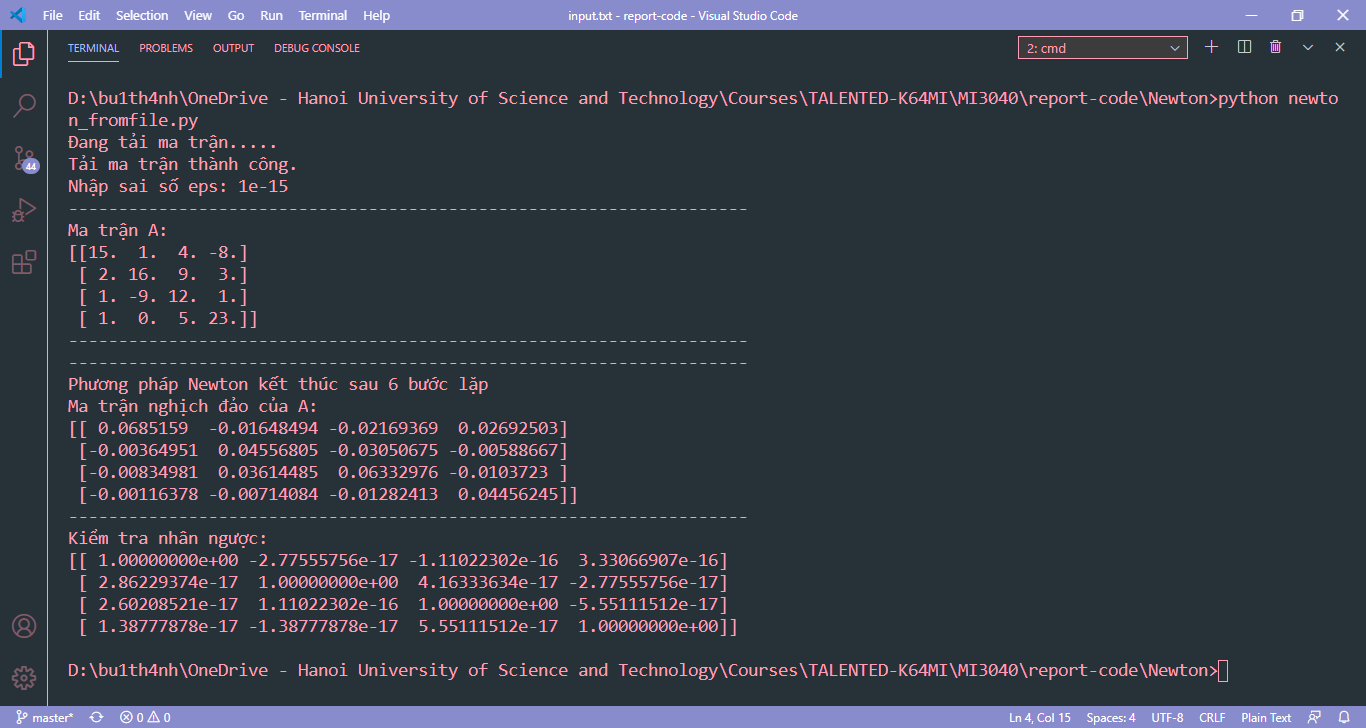
\includegraphics[scale=0.45]{example-02-newton.png} \\
        \textit{Phương pháp Newton với xấp xỉ đầu theo mục 5.2(ii)}
        
        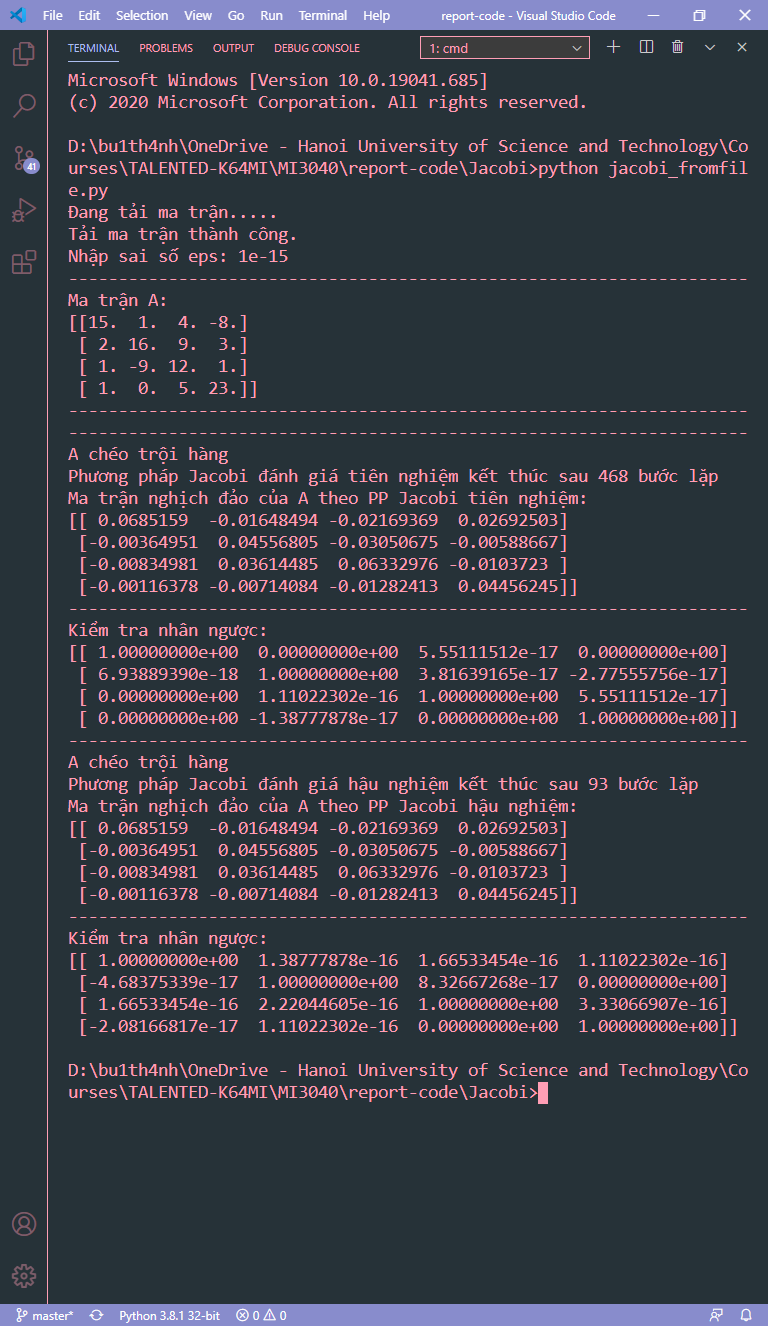
\includegraphics[scale=0.7]{example-02-jacobi.png} \\
        \textit{Phương pháp Jacobi, xấp xỉ đầu là ma trận A}
        
        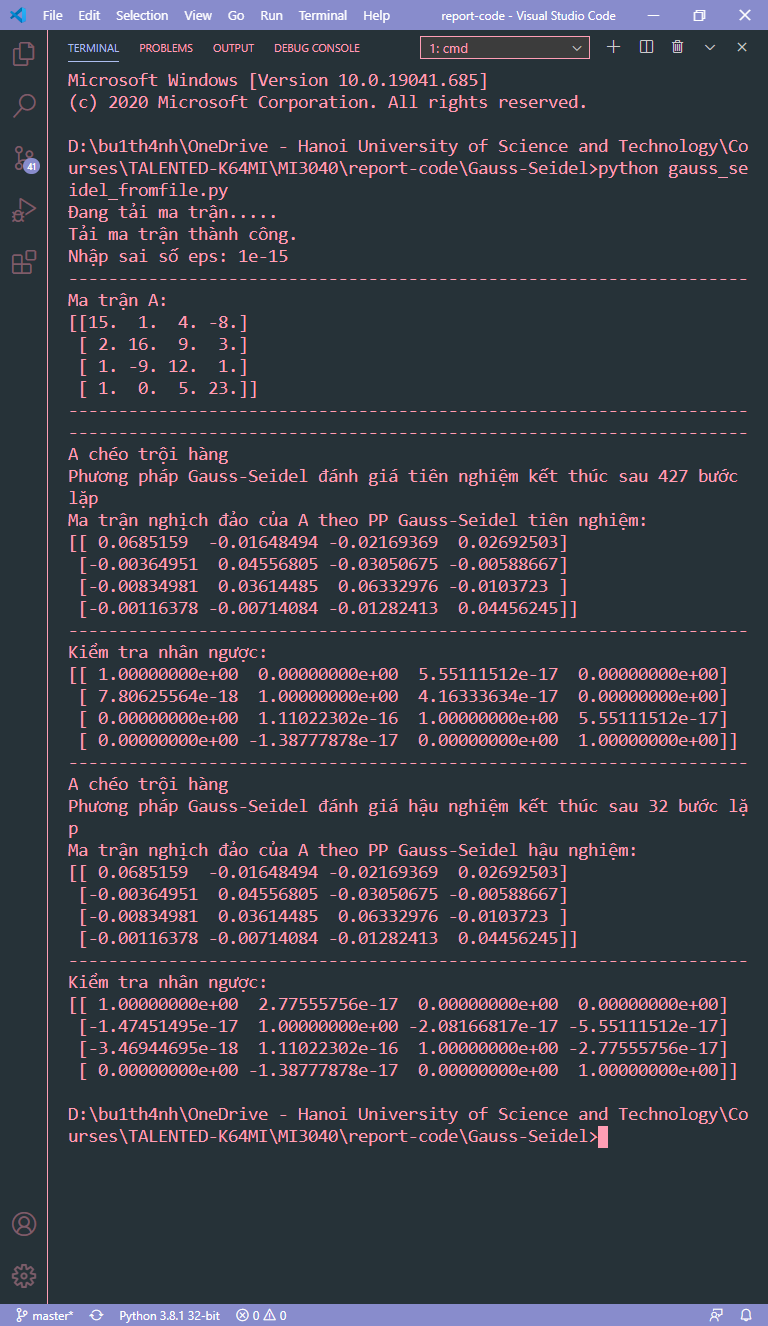
\includegraphics[scale=0.7]{example-02-gausseidel.png} \\
        \textit{Phương pháp Gauss-Seidel, xấp xỉ đầu là ma trận A}
    \end{center}

    Có thể thấy với xấp xỉ đầu là ma trận A, các phương pháp Jacobi và Gauss-Seidel có số bước lặp khá lớn do hệ số co phụ thuộc xấp xỉ đầu. Đây cũng là chủ đề nhóm sẽ cải tiến trong tương lai.
        


    \textbf{Ví dụ 2:} Nghịch đảo ma trận sau:
    $$
        \begin{bmatrix}
            0         & 5       & 0     & 0       \\
            0         & 0.00013 & 40    & 0       \\
            0         & 0       & 0.152 & 0.00067 \\
            0.00001 & 0       & 0     & 0
        \end{bmatrix}
    $$
    Đây là ma trận không chéo trội và có các định thức con chính bằng 0, tức là không thể chạy được với phương pháp viền quanh (chưa cải tiến) và các phương pháp Jacobi cũng như Gauss-Seidel. Khi chạy thuật toán Newton kèm cải tiến xấp xỉ đầu với ma trận này với sai số $10^{-15}$, ta được kết quả kèm ma trận tích của kết quả thu được với ma trận ban đầu như sau: 

    \begin{center}
        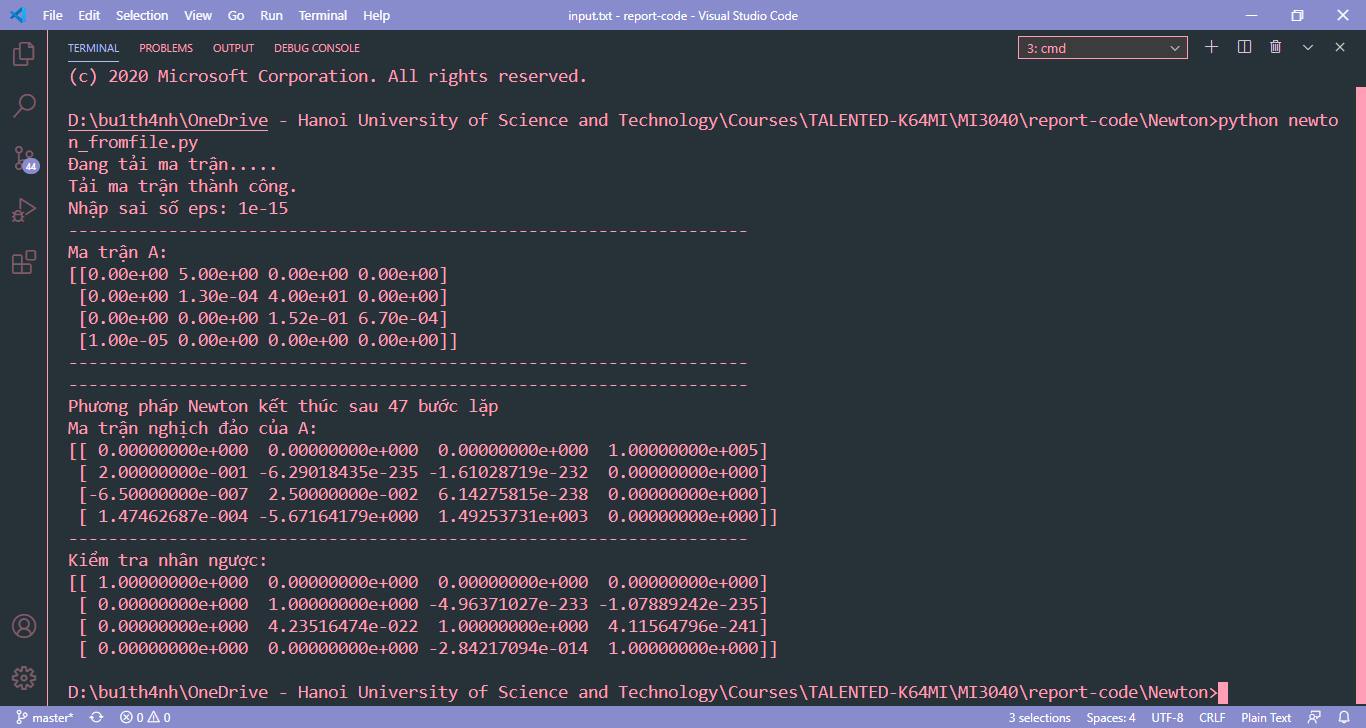
\includegraphics[scale=0.45]{example-01-newton.png}
    \end{center}


    \textbf{Ví dụ 3:} Nghịch đảo ma trận sau: \textit{(Ma trận gần suy biến)}
    $$
        \begin{bmatrix}
            3      & 2        & 7 \\
            2.0001 & 6.1      & 4 \\
            0      & 0.000001 & 0.001
        \end{bmatrix}
    $$
    Đây là ma trận chéo trội hàng và là ma trận gần suy biến, thỏa mãn điều kiện hội tụ của phương pháp Jacobi cũng như Gauss-Seidel. Khi chạy các thuật toán với ma trận này với sai số $10^{-15}$, ta được kết quả kèm ma trận tích của kết quả thu được với ma trận ban đầu như sau: 

    \begin{center}
        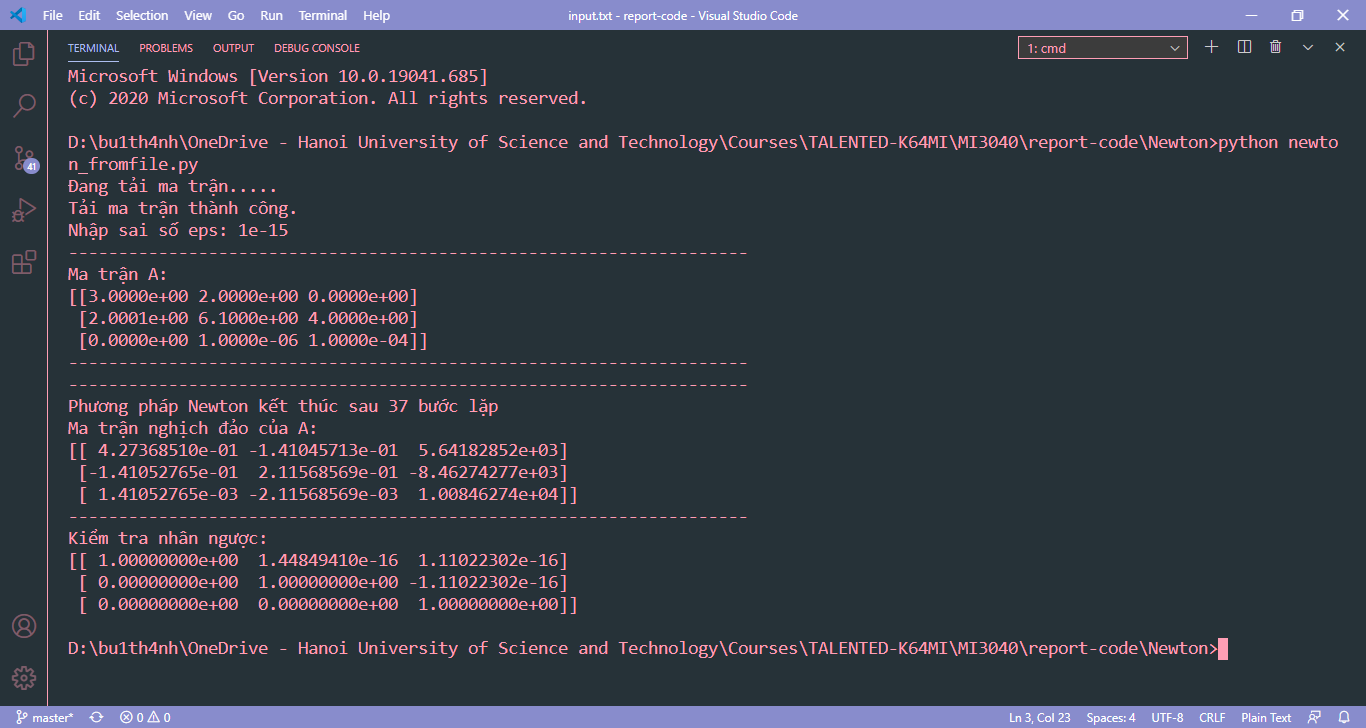
\includegraphics[scale=0.45]{example-03-newton.png} \\
        \textit{Phương pháp Newton với xấp xỉ đầu theo mục 5.2(ii)}
        
        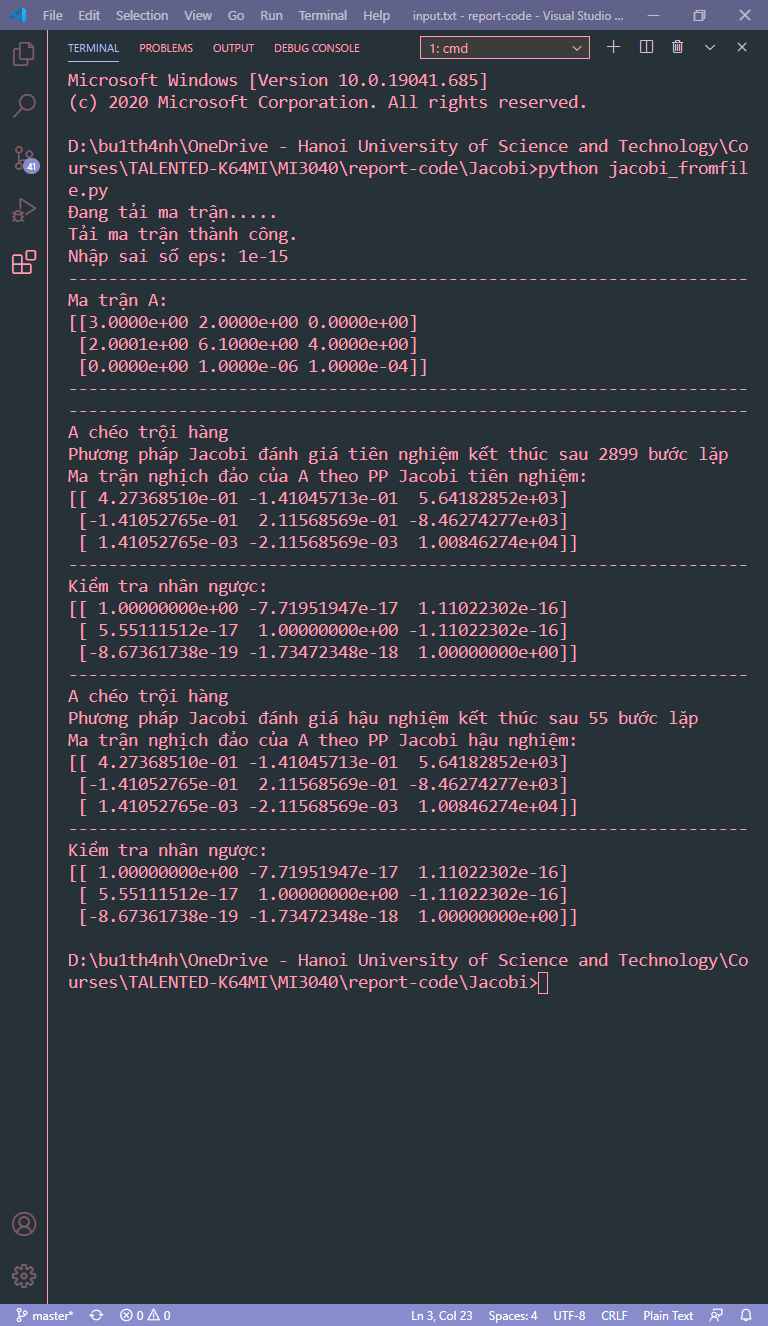
\includegraphics[scale=0.7]{example-03-jacobi.png} \\
        \textit{Phương pháp Jacobi, xấp xỉ đầu là ma trận A}
        
        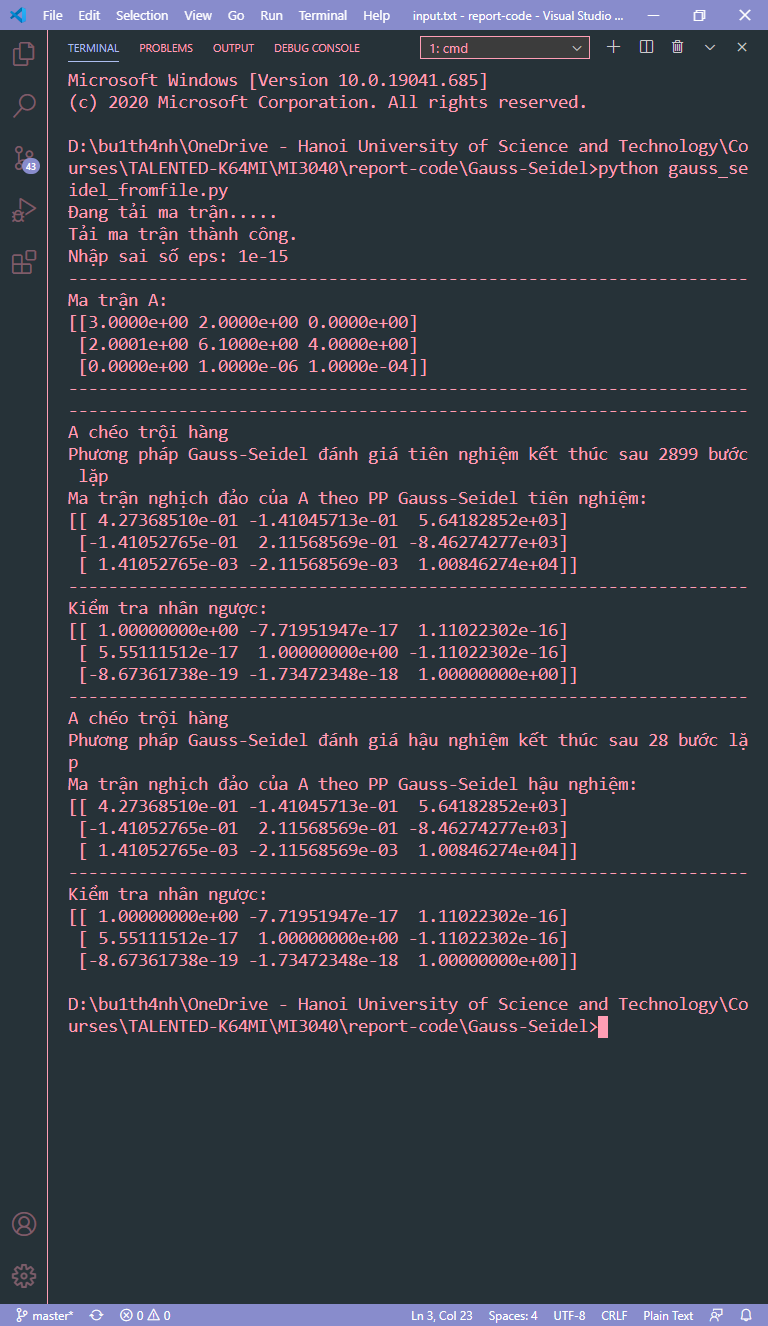
\includegraphics[scale=0.7]{example-03-gausseidel.png} \\
        \textit{Phương pháp Gauss-Seidel, xấp xỉ đầu là ma trận A}
    \end{center}

    Với hai phương pháp Jacobi và Gauss-Seidel, ví dụ này cho thấy sự khác biệt rõ rệt về số bước lặp giữa hai phương pháp tiên nghiệm và hậu nghiệm. Ở cả 2 phương pháp, cách đánh giá tiên nghiệm có số lần lặp gần 2900 bước, trong khi cách đánh giá hậu nghiệm có số lần lặp chưa đến 60 mà vẫn đảm bảo kết quả tương tự cách đánh giá tiên nghiệm. Ngoài ra, cả 3 phương pháp đều cho thấy sự ổn định khi ma trận có trạng thái gần suy biến.

\subsection{Ứng dụng}

    Nghịch đảo ma trận có rất nhiều ứng dụng trong thực tế. Chẳng hạn, có thể kể đến các ứng dụng như sau
    \begin{itemize}
        \item \textbf{Đồ họa máy tính:} Theo dõi một đối tượng trong không gian 3 chiều, có ứng dụng rất lớn trong ngành công nghiệp trò chơi điện tử, VFX và các ứng dụng VR,AR.
        \item \textbf{Kỹ thuật điện, điện tử:} Giải các hệ thống mạch điện
        \item \textbf{An toàn thông tin:} Mã hóa, giải mã thông tin
    \end{itemize}

    Đặc biệt, phương pháp Newton còn có thể sử dụng để tìm nghiệm của phương trình ma trận với ma trận hệ số không chéo trội - nhược điểm của các phương pháp lặp Jacobi, Gauss-Seidel để giải phương trình ma trận $AX = B$.
    

    \newpage
\appendix
\addappheadtotoc
\renewcommand{\thesection}{\Alph{section}}
\section{Các chương trình được sử dụng}
    \par Các chương trình trong báo cáo và slide được lưu tại các liên kết này:
    \begin{itemize}
        \item \url{https://github.com/Talented-K64MI/MI3040-Numerical-Analysis/tree/master/Topic%202.5%20-%20Matrix%20Inversion/Newton%20Method}
        \item \url{https://github.com/Talented-K64MI/MI3040-Numerical-Analysis/tree/master/Topic%202.5%20-%20Matrix%20Inversion/Jacobi%20Method}
        \item \url{https://github.com/bu1th4nh/TALENTED-K64MI/blob/master/MI3040/report-code/gauss_seidel.py} 
    \end{itemize}

\section{Mã nguồn báo cáo và bài trình chiếu}
    \par Mã nguồn báo cáo và slide được lưu tại đây: \url{https://github.com/bu1th4nh/TALENTED-K64MI/tree/master/MI3040/report}




    \newpage
    \pagestyle{plain}
    \nocite{*} % Tùy chọn cho phép in tất cả danh mục tài liệu tham khảo, kể cả tài liệu không được tham chiếu
    \printbibliography
    \addcontentsline{toc}{section}{\protect\numberline{}Danh mục tài liệu tham khảo}

\end{document}